\documentclass[11pt, openright, a4paper, notitlepage]{article}

%----------The preamble contains all the needed packages and commands (also custom commands, such as \todo{})----------------
\input{./preamble}

\begin{document}

\selectlanguage{english}
\maketitle
\vspace{4cm}
\begin{center}
\begin{tabular}{p{2cm} p{5.5cm}}
\makebox[2cm]{\hrulefill} & \makebox[5cm]{\hrulefill}\\
$^{\text{Date}}$ & $^{\text{John Doe 1}}$ \\
\\
\makebox[2cm]{\hrulefill} & \makebox[5cm]{\hrulefill}\\
$^{\text{Date}}$ & $^{\text{John Doe 2}}$ \\
\\
\makebox[2cm]{\hrulefill} & \makebox[5cm]{\hrulefill}\\
$^{\text{Date}}$ & $^{\text{John Doe 3}}$ \\
\\
\makebox[2cm]{\hrulefill} & \makebox[5cm]{\hrulefill}\\
$^{\text{Date}}$ & $^{\text{John Doe 4}}$ \\
\\

\end{tabular}
\end{center}
\thispagestyle{empty} \newpage
\newpage
\thispagestyle{empty}
\mbox{}
\input{./Title}
\newpage
\thispagestyle{empty}
\mbox{}
\pagenumbering{roman}
\setcounter{page}{0}
\input{./text/preface}
\newpage
\thispagestyle{empty}
\mbox{}
\newpage \tableofcontents
\newpage
\mbox{}
\newpage
\onehalfspacing

\pagenumbering{arabic}
\setcounter{page}{1}

\section{Introduction}
\label{sec:introduction}
Netflix is a streaming service that provides access to many movies and series for a monthly subscription fee. The initial idea was to have a single place for all the movies and series, but some companies withdrew their licenses to create their own streaming services. The net result is that there now are many streaming services who each require their own subscription and who each provide access to a smaller number of movies and series.

Our Business idea is: to have a collected service that provides access to all, or at least many, of the streaming services through a single client and with a single larger subscription fee. To be competitive on the price we will rely on working out some deal with the included streaming services that allows us to pay them from our subscription money dependant on usage of their service.
\section{Business Idea}
\label{sec:idea}
Our idea has been given the working title ``Watchr''. The intention is to collect all streaming services\footnote{We will refer to streaming services providing movies, series and TV shows as simply ``streaming services''} into a single interface. This interface will serve as a gateway to the different services, providing access to their shows.

To elaborate on the idea, we want to analyse it and its market. For this, we have used some existing models, being Porter's Five Forces and resource-based theory. This section will elaborate on each of the mentioned methods, as well as covering the blue and red ocean strategies.

\subsection{Porter's Five Forces}

Using Porter's Five Forces, we can analyse the market, and how it affects our product. As we deem the market dangerous, as it is occupied a lot, we believe this business model can be useful for the process. Figure \ref{fig:five_forces} is a visual representation of the model, where our considerations are pointed out for the forces. Each of these will be further explained.

\begin{figure}[h]
    \begin{center}
        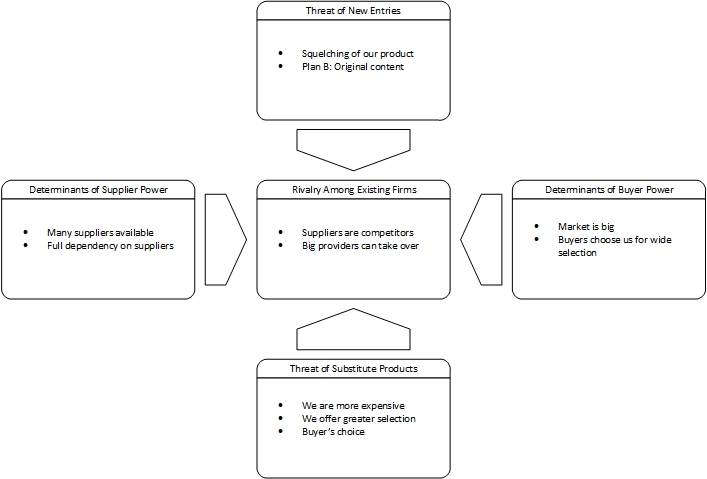
\includegraphics[scale=0.65]{./pics/five_forces}
        \label{fig:five_forces}
        \caption{Porter's Five Forces for the project}
    \end{center}
\end{figure}

\subsubsection*{Determinants of Supplier Power}
The suppliers for the project are providers of motion pictures through streaming over the internet. There are many of these providers, which is the main reasoning for the project. For the project to succeed, these providers must agree to supply the project. This causes a thread, as we then become very dependent on the suppliers. There also exists the thread of the suppliers becoming too big, challenging our idea.

\subsubsection*{Determinants of Buyer Power}
As there already exists providers for motion pictures through streaming that are thriving, it can be concluded that the market exists, but is risky to enter. Our product differs in our wide range of selection, as we serve as a gateway to the existing companies, and do not quelch the existing market. The hope is that users will choose us for this quality, and that we can capture the part of the market that want to use several services, but don't want to pay for them all.

\subsubsection*{Thread of Substitute Products}
The services that exist for the market are not combining the effort of all suppliers, which gives us both an advantage and a disadvantage: As we are a gateway to existing services, we offer a greater selection, but we are therefore also more expensive. The greatest thread of a substitute is if an existing provider expands to the point that we are not needed as a service.

\subsubsection*{Thread of New Entries}
If a new competitor is to enter the market, a possible outcome is loss of suppliers. Imagine this scenario: The new competitor will gain suppliers, possibly by focusing on our product's weak points, and perhaps gain some of our suppliers as well. As there is a risk involving loss of suppliers, a natural backup plan would be to create media of original content. If our suppliers are then lost, we will simply become another streaming service. To avoid this, we must focus on our weaknesses, and make sure we are never seen as the second best choice for suppliers.

\subsubsection*{Rivalry Among Existing Firms}
One of the problems in this business is the fact that the suppliers can be seen as competitors. They are suppliers, but they are not dependent on us, although we are completely dependent on them in the start. The greatest streaming services are very successful in themselves, and if they become too big, we are not needed as a service.

\subsubsection*{Discussion}
The market itself is greatly occupied, which is both positive and negative. On one hand, we might be an unnecessary service. On the other hand, we offer a collection of the existing services, for ease of access and saving of money. The dependency on our suppliers is a risk, as we can only succeed in this project if a set of providers agree to supply access. The market itself is therefore a difficult one, as we twist it to our advantage, but at a great risk.
\subsection{Resource-based theory}

Generally, a company could be perceived as a collection of resources and certain capabilities which defines the resource-based theory of the company \cite[p. 13-14]{fiveForces}.
When these resources are combined in the right way, they form organizational capabilities.

In our case, we try to combine technically talented people (software developers and engineers, system architects, UI and integration specialists) and the appropriate software tools with the collaboration of streaming services (through the use of the media patents they have on specific tv series, movies etc.) in order to create a competitive advantage. This competitive advantage is described by the idea that our platform will provide access to media from several streaming services in one place with the use of only one subscription and the option to watch specific shows from these.

The key resources we consider for our company are as follows:

\begin{enumerate}
  \item \textbf{Brand}\\
In business, branding plays a pivotal role in defining a company. A company's brand is what differentiates and distinguishes it from its competitors and what makes it stand out across as unique and established. 
A company communicates with its customers through its brand, a promise which relies the information of what products and services they can expect. Microsoft, Apple, Samsung and many other companies are easily recognized through their logos and the products and services they provide. In our case, we build the company around our media unifying platform ``Watchr'' where both the company and the platform have distinguishable and unique logos.

  \item \textbf{Software Products}
  
  	\begin{enumerate}
   		\item \textbf{Platform}\\
Currently, our business plan revolves around Watchr, our media platform and its success is essential for the success of the company as a whole.
	    \item \textbf{Algorithms and protocols}\\ 
The underlying structure of Watchr will build upon proprietary algorithms and specific protocols which will be used for establishing the right user experience for our customers. An example of such could be a recommendation system adapting based on users' preferences, sorting and filtering algorithms for different criteria. 
    	\item \textbf{Hardware}\\
Similarly to how our competitor's media streaming services work, we would have dedicated physical servers for storing all the content on Watchr along with all the user-related information. As a positive note, we do not have to store movies and such on the servers, as this information is gained from the suppliers.
  	\end{enumerate}
  \item \textbf{People/Talent}\\
People are the most important resource for a company in order to function correctly and be successful. Since we are building a media platform, we need people with technical expertise in programming, system design,architecture and integration. Additionally, we would need people with the right aptitude to maintain the system and project managers to guide and manage everyone else with further development and new features.
  \item \textbf{Core Competencies}
  	\begin{enumerate}
        	\item \textbf{Software processes and methods}\\
In order to implement Watchr, the technical people in the company should adhere to a software development methodology and use specific software processes to facilitate that. A good choice would be an iterative approach such as SCRUM.
        	\item \textbf{Knowledge}\\
The knowledge a company has access to is another valuable commodity. In our case this can include all from technical expertise and business knowledge about the market to social relations with partners and other companies.
        	\item \textbf{Community}\\
A company which has direct access to its community, or namely its customers, can greatly benefit from its feedback on certain features of the product or service at hand, as well as how some parts could be improved and revised. Therefore, a good idea would be to implement a direct way for our customers to contact us through Watchr.
    \end{enumerate}
  \item \textbf{Vision Direction}\\
The ongoing vision of the company is to unite all the streaming media available on other separate platforms in one place which will facilitate the access for everyone to his/hers favourite tv shows, series etc.
\end{enumerate}

These resources can be added to certain capabilities of the company, which in turn will define its competitive advantage. The defining capabilities in our case are:

\begin{enumerate}
  \item Learn new programming skills
  \item Deliver quality through our platform and services
  \item Respond to feedback and customer needs
  \item Expand existing features and develop new ones
\end{enumerate}
\subsection{Blue And Red Ocean}

Red oceans and Blue oceans make up the market universe, as defined by \textit{Kim} and \textit{Mauborgne} \cite{Blue_ocean_strategy}. Red oceans cover all the existing industries and businesses (known market space), and the Blue oceans cover the ones which are not created yet (unknown market space), respectively.

We consider our company to be mostly in Red ocean territory because Red ocean strategy is a market-competing strategy, and we would build our platform on the premise of using media provided by our competitors, with an already established market rules. We say mostly, not entirely, since our platform will have a bit of novelty where nobody else  has created such a platform so far to effectively unify this type of media streaming content. This falls under the description of Blue ocean strategy where something new is created within red oceans territory by expanding existing industry boundaries.
\section{Business Model Canvas}
\label{sec:business_canvas}
In this chapter we will discuss the business canvas model for our idea, as well as pattern considerations and our design approach.

By building up a business model canvas as a concept for our project, we gain insight for discussion, and a common understanding for what we are doing. Using Osterwalder's approach \cite[p. 1-51]{canvas}, this is done through nine building blocks. In \figref{fig:model_canvas}, a graphical overview of the nine blocks can be seen. Each will be described with relation to the project throughout this chapter.

\begin{figure}[h]
    \begin{center}
        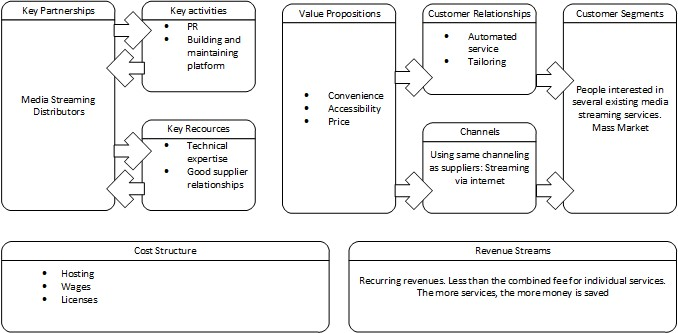
\includegraphics[scale=0.8]{./pics/model_canvas}
        \caption{The Business Model Canvas for our project}
        \label{fig:model_canvas}
    \end{center}
\end{figure}


\subsubsection*{Customer Segments}
Our product aims for an already existing market, although we want to change this market. Nonetheless, it is a mass market, consisting of people interested in several existing media streaming services.

\subsubsection*{Value Propositions}
We are focusing on the customers, who seeks several streaming services, collected in one place and at a lower price. That means there are three services of value for the customers: Convenience, accessibility and price. Convenience comes in collecting the product in one place, and making the interface painless to use. Accessibility is in the amount of suppliers, as more suppliers give wider range of streaming possibilities. Pricing lies in how far down we can push the price, which is also dependent on the suppliers, among other possibilities, such as advertisement.

\subsubsection*{Channels}
There are several ways of reaching our customers. The one way we are sure of is the fact that we want to offer our services through the same experience as existing services offer them: Streaming over the internet. It is important to note that this has to be done over several platforms, to gain competitive value through accessibility. This includes applications for mobile devices and for consoles. Advertisement of our product can be done in several ways, but one of the least costly ways to go about this is through the suppliers. As the customers are those already using the services that our suppliers offer, the best place to advertise is through these.

\subsubsection*{Customer Relationships}
As the existing companies do, being the suppliers of our product, we want to offer an automated service through a personal profile. Through this, it is possible to offer service without greater work effort, as well as the customer being able to mend their profile to their needs. As an extra feature, we want the customer to be able to tailor their own profile to their needs. They should only have access to and pay for the services needed, in the case they only want a subset of supplier services. With personal profiles, it is possible through algorithms to use knowledge on past activity to aid the user in their experience and to suggest future actions. If a customer seems to never use the services from a specific supplier, then we can give awareness of this, such that the user can tailor the profile further.

\subsubsection*{Revenue Streams}
Through the personal profile as an automated service, we want to create earnings through subscription fees. As the most successful streaming services have their income through this method, we see no reason to change this. We want to tempt customers to use our service by being cheaper than using all the services of the customers separately. Furthermore, to tempt customers to buy more, they are given greater offers the more suppliers they add to their profile.

\subsubsection*{Key Resources}
The most important resources for this project is partnerships with the suppliers and technical expertise. If we do not have suppliers, we don't have a service. If we do not keep the suppliers satisfied with our partnership, we lose them again. Technical expertise ensures a good, reliable client for the customers. The most needed resources are therefore intelligent and human resources.

\subsubsection*{Key Activities}
As the business comes up and running, the main activity is maintenance in both relationships and in customer support. If we do not continue our partnership with the suppliers, we cannot guarantee our main contribution from the service, and therefore lose customers. If the customers are unhappy with the product, we will lose them if we aren't able to locate and handle the problem.

\subsubsection*{Key Partnerships}
The media streaming distributors are our main suppliers, as they give access to the motion pictures our customers want to see. without these, the rest of the business will crumble. It is worth to note that this creates a great risk, as if we cannot live up to the expectations of our suppliers, we can lose these.

\subsubsection*{Cost Structure}
There are three major cost factors for this project: Hosting, wages and licenses. We need hardware, software locales and technical expertise for hosting our client. As we need expertise in some areas, such as marketing, there is a greater cost in waging. Furthermore, there is the licensing cost, as we must pay the suppliers for their service to us. We want to handle this as a percentile split, depending on the individual customer. A certain amount from each subscription is dedicated to the suppliers. The amount is based on how the customer has tailored the profile, and how much this individual is paying. Depending on what supplier services the customer has been using, the amount of money is then split, to give those that contribute to the individual customer a greater share of the profit. Another way is to make a fixed arrangement with each supplier, giving the possibility of a greater content variety, and therefore a greater attraction value for new customers.

\subsection{Pattern Considerations}
There generally exists five categories of business model patterns\cite[p. 52-119]{canvas}:
\begin{itemize}
\item Un-Bundling Business Models
\item The Long Tail
\item Multi-Sided Platforms
\item FREE
\item Open Business Models
\end{itemize}

The pattern to consider regarding our business idea is mostly the The Long Tail pattern where elements from the Multi-Sided Platform patterns can be used. Parts from the Open Business Models are also worth considering, as a lot of inspiration can be gotten from already existing services (HBO Nordic, Netflix, etc.), but that is strictly speaking not necessarily \emph{collaborating with outside partners}\cite[p. 109]{canvas}, so the consideration is on the other two.

The most fitting pattern is the Long Tail, as we want to provide both ``non-hit'' and ``hit'' products to all of our customers. It makes sense as our business idea fits mostly to the points presented in \emph{Business Model Generation}\cite[p. 75]{canvas}. Another hint that this pattern is the best fit for the project is the fact that our service is similar to Netflix and they used the Long Tail pattern. At least they used to, it seems like they are moving away from ``non-hit'' products and producing their own ``hit'' TV shows (House of Cards, Orange Is the New Black, etc.). The elements from the Multi-Sided Platforms that can be used are regarding the revenue stream, as we can possibly do a similar deal as Spotify and Telia. Telia provides with their mobile plan a Spotify subscription. If we can get a similar deal, the revenue loss can be subsidized by customers of our own service, but we will possibly reach a larger market.
% 1: Business model generation, 52-119
% 2: Business model generation, 109
% 3: Business model generation, 75
\subsubsection{Design Approach}
We have chosen to use the Customer Insight\cite{1} techinique in our design approach. If we had the funds available, we could hire social scientists which could sketch profiles of the customer segment. As this is not the case, we have made use of the Empathy Map, which is also known as the ``really simple customer profiler''\cite{2}.

The first thing to do when using the empathy map, is to brainstorm all possible customer segments that one might want to serve with the business model. Then three promising candidates should be chosen, from which one is selected for the first profiling exercise. Then a customer from that customer segment is thought up, by giving the customer characteristics, such as a name, income, occupation, and so on. Afterwards a profile is build for the customer by asking and answering six questions.
These questions should be put on a whiteboard or flipchart, as seen in figure \ref{fig:empathy_map}(Hence, empathy map), and the answers could be written on stick-it notes and placed on the questions.

% 1: Business model generation, 127-133
% 2: Business model generation, 131
\section{Paradigms}
\label{sec:paradigms}
In this chapter we will discuss the software entrepreneurship paradigms and outline how we use one.

For software entrepreneurship we consider the two paradigms from \textit{Software	Entrepreneurship}\cite[p. 27-39]{Software_entrepreneurship}: Analyse, Design, Enact (ADE) and Consider, Do, Adjust (CDA).
The ADE paradigm relies on causal logic with a focus on predicting the future to control it.
It is a useful paradigm when the future is knowable, the goal is clear and the environment is reasonably well structured.
The CDA Paradigm instead relies on effectual logic with a focus on working with the things that can be controlled.
It is a useful paradigm when the future is unknowable, the means are clear, and the environment is subject to human shaping.

For our project we have a clear goal (a collection of streaming services), but are not sure which means we have available (which kind of agreement we can make with streaming services).
Furthermore, the environment is well structured with several other subscription streaming services to compare with, and use the comparison to get an idea of the future.
Therefore we choose the ADE paradigm.

When outlining the business process we use the business model design process from \textit{Business Model Generation}\cite[p. 244-261]{canvas}. %the page number is from the index of the preview as I don't have the book
We consider it five phases rather than activities because we use the ADE paradigm.

\subsection{Mobilize}
In the mobilization phase we would assemble our team, which would consist of us as programmers and some sales specialist. It might also be a good idea too contact some streaming services to test the preliminary business idea.

\subsection{Understand}
The primary action for us in the understanding phase would be to research the existing streaming services. Their pricing and assortment would give us a better idea of our potential market position, and analysing their client features would give us an idea of expected features for our client.
If we are in contact with the streaming services at this point we can also use their expert knowledge on the area.
Since our intended product is very similar to existing products with an established market, we are unlikely to get much out of studying potential customers.
%maybe something about netflix as an earlier failure

\subsection{Design}
In this phase we would probably focus on designing various business ideas and propositions for the streaming services. We might also make a prototype of our client.

\subsection{Implement}
Here we will contact the streaming services and negotiate an agreement with them based on our business ideas. We would then implement the system based on the agreement.

\subsection{Manage}
The manage phase is mostly a maintenance phase for our business. Here we could very well switch over to an iterative or agile approach as we focus on keeping our product the best through continuous improvement.

\subsection{Financial Issues}
Our biggest financial issue is that if we don't get a good agreement with the existing streaming services we will have difficulties being price competitive. We can make a vendor service that simply provides the convenience of browsing the services you have already paid for, but it is difficult to get much profit out of it. Either we charge for using our service which would make the total cost inarguable worse, or we use advertisements which risks hurting the convenience we sell our product on.
\section{Related Work}
\label{sec:related_work}

In this chapter, we have chosen two papers to relate theories from to our business idea and the Watchr media platform. The papers in question are: "\textit{The Early Stage Software Startup Development Model: A Framework for Operationalizing Lean Principles in Software Startups.}" (Bosch, Bjork and Ljungblad) and "\textit{The Nature of the Entrepreneurial Process: Causation, Effectuation, and Pragmatism.}"(Kraaijenbrink). 

\subsection{The ESSSDM}

Contrary to popular belief, many software start-ups fail in their inception and there are only a very few that manage to become very successful (Facebook, Twitter, Instagram to name a few). In order to identify what factors contribute to the success of a software start-up, we first have to understand what constitutes one. According to Ries \cite{leanStartup}, a "\textit{startup is a human institution designed to deliver a new product or service under conditions of extreme uncertainty}". Additionally, many start-ups usually have limited resources in terms of people and funding at their disposal, which strengthens the importance of minimizing the development time and effort while maximizing the value. Lean principles emphasize on continuous learning through customer validation and short feedback cycles to identify which efforts or activities generate customer value.

In order to address that, we would make use of the Early Stage Software Startup Development Model (ESSSDM) \cite{bosch} and elaborate on each of its comprising parts. A visual representation of the model can be seen in \figref{fig:esssdm}. This model allows the exploration of multiple ideas in parallel and evaluating the ones worth scaling through short iterative cycles (using the Build-Measure-Learn loop). It consists of three parts: 
  
\begin{figure}[h]
\begin{center}
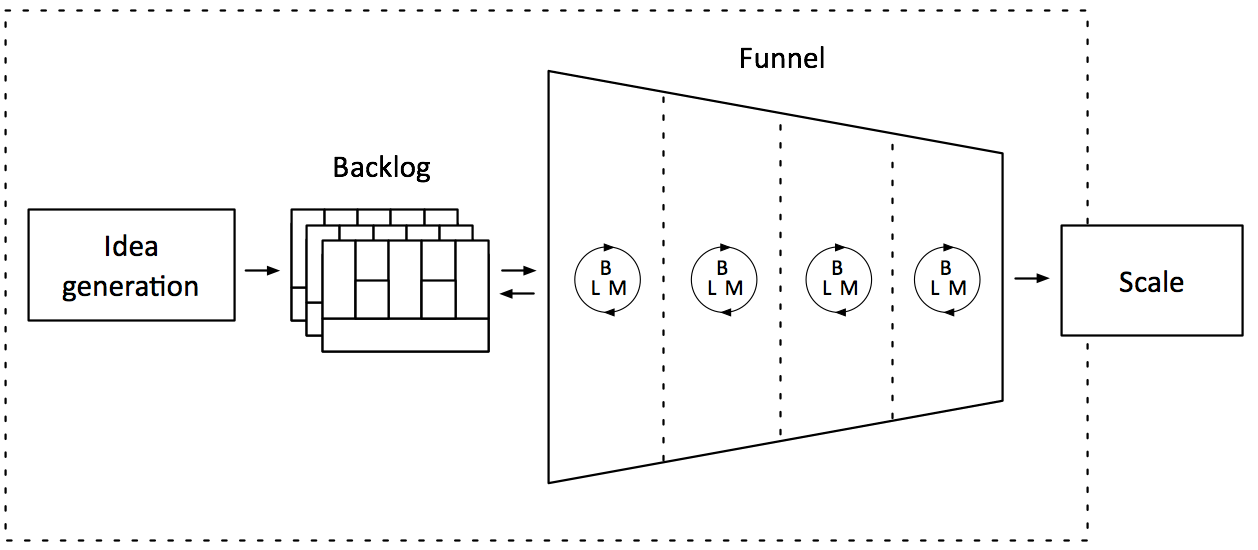
\includegraphics[scale=0.55]{./pics/ESSSDM}
\caption{Early Stage Software Startup Development Model}
\label{fig:esssdm}
\end{center}
\end{figure}

\begin{enumerate}
\item Idea generation

This stage is considered a part of the startup process and happens prior to incorporation. In our case, we started by brainstorming several possible avenues we can pursue before eventually settling on building an online media streaming platform, which would incorporate some elements from already existing platforms (content filtering by different criteria, recommended, popular and favourite lists, rating system etc.). 
\item Ideas backlog

Here is where all the ideas generated are put into a prioritized backlog. It is really important that they are written in comparable format otherwise the prioritization  becomes extremely complex. Some other product ideas we have included:
\begin{itemize}
    \item An ``Omni-compiler'', which would conceptually make it possible to translate between any programming languages
    \begin{itemize}
        \item A minor idea would be a compiler which would conceptually translate legacy COBOL code, heavily used in the financial sector and with a high demand, into a modern language
    \end{itemize}
    \item A mobile game with a competitive nature given the current high market demand
\end{itemize}
\item The Funnel

The last stage of the ESSSDM entails how multiple ideas are fed into a "funnel" where they undergo a validation systematically by the use of the Build-Measure-Learn (BML) loop. Multiple ideas can be in the funnel while being validated in parallel. This is worthwhile since it is really important to stay objective in the early stages of a startup. This gives an open mind and willingness to change instead of sticking and growing attached to one single idea which might be damaging that early on. This stage consists of four sub-stages: (1) Validate problem, (2) Validate solution, (3) Validate Minimum Viable Product (MVP) small-scale, and (4) Validate Minimum Viable Product (MVP) large-scale. Since the validation and a MVP is beyond the scope of this project, we do not address the four stages.
 \end{enumerate}
 
\subsection{The Nature of Entrepreneurial Process}
\label{sec:gote}
Jeoroen Kraaijenbrink has made a paper on the entrepreneurial process \cite{kraaijenbrink}. The focuses on the dimensions of the different models rather than the models themselves, as well as a suggestion on connection the nature of entrepreneurship with the nature of human actions. The connection to the human actions is mostly a suggestions, with a few relations to how the human actions are biased. We will talk about our idea in relation to the dimensions mentioned in the paper. Furthermore, We bring a suggestion to an extended version of this model, combining the model with a cognitive process.

\subsubsection*{Dimensions}
As the paper suggests, the process can be tailored in many different ways, as there is no single correct process. Our project is based on an idea, and how this idea can be brought to life. On first glance, this is a ends-driven process, but it can easily be tailored as a means-driven process. This would cause the means to be of more value than the goal, and the goal is open for change. What cause is taken is based on whether we have an affection to Watchr as a service, or it is the entrepreneurial process and the final expectations that have focus.

The most certain of the dimensions for this project is the fact that it focuses on cooperation with existing companies. If we only compete with the market, we will have no suppliers.

The service we are creating is focused on an existing market. The service itself is new, yet its content is already existing. Netflix is the closest to an existing service with the same capabilities, and we try to take this idea even further. To this extend, we are creating an existing service to an existing market, but it can be argued that the service itself is new.

If we try to predict the outcome of the service in hope of controlling the process, we should focus on the existing market. The users should be found to some extend, and whether these are willing to pay for our service. On the other hand, if we control in order to avoid the need to predict, we should focus on previous models for existing and thriving services. Although we can be seen as a new service, we are in an existing market, which makes it possible to gain a certain level of control.

It is a fact that the service is most successful if we have all streaming services available. But the cost for obtaining this level of service, it comes at a great cost. The question is whether we are able to walk away unharmed in case the project fails. The dimension choice of either expecting good results or only commit what we can afford to lose is important, yet hard to make. It is a subjective choice, which depends on the management for the project, and the likeliness of success.

\subsubsection*{GOTE}
G.O.T.E. is an acronym created by Robert Cohen and a method used in theatre and drama \cite{gote}. The method is normally used for reminding the actor of four elements needed when creating a character and its situation. The acronym is for \emph{Goal}, \emph{Obstacle}, \emph{Tactics} and \emph{Expectations}. The goal is what the character desires, the obstacle is what hinders the character in achieving the goal, the tactic is the method used to achieve goals, and the expectation is what the character expects to achieve if succeeding. We believe the method is also suitable for entrepreneurship to create a ends-driven model based on methods rather than specific models.

The GOTE can be used to describe processes in entrepreneurship on a high level, as seen on \figref{fig:gote}. The ultimate goal is to create a product or a service. Several obstacles stands in the way, which are found through existing models, such as Porter's Five Forces. The tactics are a list of ways to overcome the obstacles. The expectations of the goal is often to gain money, although it sometimes is for the thrill of the process and satisfaction in seeing the end goal.

\begin{figure}[h]
\begin{center}
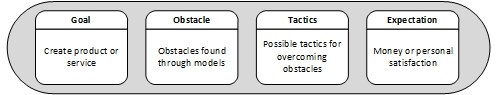
\includegraphics[scale=0.7]{./pics/gote}
\caption{The GOTE method used in entrepreneurship on high level}
\label{fig:gote}
\end{center}
\end{figure}

An interesting take on the GOTE method is the fact that it works on several layers, in both acting and entrepreneurship. This means using the tactics as a new goal, and finding obstacles and tactics for this goal. The expectation for the goal is to come closer to the upper level goal. An example for this in relation to our project can be seen in \figref{fig:gote_watchr}.


\begin{figure}[h]
\begin{center}
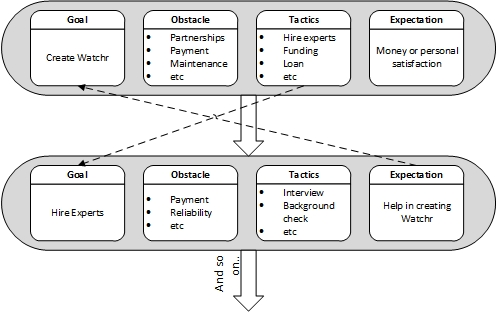
\includegraphics[scale=0.7]{./pics/gote_watchr}
\caption{The GOTE method used several layers for Watchr}
\label{fig:gote_watchr}
\end{center}
\end{figure}

The GOTE method used in entrepreneurship is an ends-driven approach, as it focuses on the goals and expectations. It is linear, as it has little to no possibility in iterations in itself. Apart from these factors, it is possible to use this approach in many aspects, as it is only a tool for process. It is based mainly on concrete situations, and finds the difficulties and obstacles through corporeality. To overcome these difficulties, tactics are found through sociality.



%-------------Write references in the references.bib file. An example is given in the file (or just google)----------------
\section{Bibliography}
\cleardoublepage
\phantomsection
\addcontentsline{toc}{chapter}{Bibliography}
\bibliographystyle{ieeetr}
\bibliography{./text/references}{}
\newpage
\mbox{}

%-------------------------Appendices part if needed-------------------
%\newpage
%\part{Appendices}
%\appendix
%\input{./text/appendix}

\end{document}